\documentclass[12pt, a4paper]{article}

\usepackage[utf8x]{inputenc}
\usepackage[greek, english]{babel}
\usepackage{caption}
\usepackage[section]{placeins}
\usepackage{balance}
\usepackage{dblfloatfix}
\usepackage{hyperref}
\usepackage{color}
\usepackage{graphicx}
\usepackage{float}
\usepackage{tikz}
\usetikzlibrary{shapes.geometric, arrows}
\tikzstyle{stage} = [rectangle, rounded corners, minimum width=3cm, minimum height=1cm,text centered, draw=black]
\tikzstyle{arrow} = [thick,->,>=stealth]



%\usepackage[margin=2cm]{geometry}
%\usepackage{graphicx,wrapfig,lipsum}

\newcommand{\en}{\selectlanguage{english}}
\newcommand{\gr}{\selectlanguage{greek}}

\hypersetup{
	colorlinks=true,
	linkcolor=blue,
	filecolor=magenta,
	urlcolor=blue,
}

\begin{document}
	
\gr
\begin{titlepage}
	
	\begin{center}
		\vspace*{0.5cm}
		
		\LARGE
		\textbf{\normalsize ΑΥΤΟΜΑΤΗ ΚΑΤΑΤΜΗΣΗ ΚΑΙ ΚΑΤΗΓΟΡΙΟΠΟΙΣΗ ΤΗΣ ΠΟΛΥΔΙΑΣΤΑΤΗΣ ΧΡΟΝΟΣΕΙΡΑΣ ΑΙΣΘΗΤΗΡΙΑΚΩΝ ΣΗΜΑΤΩΝ}
		
		\vspace{0.5cm}
		%\LARGE
		%\Large 
		%\gr{}
		
		\vspace{1.5cm}
		
		\textbf{Γεώργιος Βαρδάκας}
		
		\vfill
		
\includegraphics[width=0.5\textwidth]{logo.png}
		
		\textbf{\normalsize Επιστημονικός υπεύθυνος έργου: \\ Στέργιος Αναστασιάδης (Αναπληρωτής Καθηγητής)}
		\vfill
		
		\vspace{0.8cm}
		
		\Large
		Τμήμα Μηχανικών Η/Υ και Πληροφορικής\\
		Πολυτεχνική Σχολή Πανεπιστημίου Ιωαννίνων\\
		%Ελλάδα\\
		\date{\today}
		
	\end{center}
\end{titlepage}


\tableofcontents
\newpage

\gr
\section{Εισαγωγή}
Στην παρούσα εργασία κληθήκαμε να λύσουμε το πρόβλημα της αυτόματης κατάτμησης και κατηγοριοποίησης της πολυδιάστατης χρονοσειράς αισθητηριακών σημάτων στα πλαίσια του έργου {\bf "\en HOMORE:\gr ΕΞΥΠΝΟ ΣΥΣΤΗΜΑ ΠΑΡΑΚΟΛΟΥΘΗΣΗΣ ΤΗΣ ΦΥΣΙΟΛΟΓΙΚΗΣ ΔΙΑΒΙΩΣΗΣ ΗΛΙΚΙΩΜΕΝΩΝ ΣΕ ΑΣΤΙΚΕΣ ΚΑΙ ΑΓΡΟΤΙΚΕΣ ΠΕΡΙΟΧΕΣ"} με κωδικό {\bf 82475}. Για να το πετύχουμε αυτό αρχικά συλλέχθηκαν τα δεδομένα που είναι απαραίτητα για την κατασκευή ενός μαθηματικού μοντέλου μηχανικής μάθησης, και στην συνέχεια ακολούθησε η προ-επεξεργασία τους, ώστε να είναι κατάλληλα προετοιμασμένα για να εισαχθούν στο μοντέλο. Επιπρόσθετα μελετήθηκαν διάφορα μοντέλα μηχανικής μάθησης, μέχρι να βρεθεί αυτό με τα καλύτερα αποτελέσματα. To τελικό μοντέλο περιέχει εσωτερικά τα βήματα της προ-επεξεργασίας αλλά και της πρόβλεψης με αυτόματο τρόπο και βασίστηκε σε μεγάλο βαθμό στην μεθοδολογία \cite{arXiv:1802.01489}. Τελικά η αξιολόγηση του μοντέλου μηχανικής μάθησης για τον έλεγχο της ποιότητας των αποτελεσμάτων του πραγματοποιήθηκε με \en (group) K-fold cross validation\gr. 

\section{Συλλογή Δεδομένων}
Μία προαπαίτηση για την κατασκευή ενός μαθηματικού μοντέλου μηχανικής μάθησης είναι φυσικά τα δεδομένα, καθώς αυτές οι μέθοδοι μαθαίνουν μέσα από αυτά. Για την συλλογή των δεδομένων έγινε χρήση του έξυπνου ρολογιού \en Fitbit Versa\gr. Το έξυπνο αυτό ρολόι, μας δίνει την δυνατότητα να αντλήσουμε τις μετρήσεις που καταγράφουν οι διαθέσιμοι αισθητήρες του. Οι αισθητήρες αυτοί αποτελούνται από από το γυροσκόπιο, το επιταχυνσιόμετρο καθώς και τον αισθητήρα καρδιακών παλμών. Οι αισθητήρες του γυροσκοπίου και του επιταχυνσιομέτρου καταγράφουν μετρήσεις με συχνότητα $10$ \en H \gr ενώ ο αισθητήρας καρδιακών παλμών καταγράφει μετρήσεις με συχνότητα $1$ \en H\gr. Στην παρούσα εργασία έγινε χρήση μόνο των αισθητήρων του γυροσκοπίου και του επιταχυνσιομέτρου καθώς οι καταγραφές του αισθητήρα των καρδιακών παλμών δεν περιείχε χρήσιμη πληροφορία για την αυτόματη κατηγοριοποίηση της πολυδιάστατης χρονοσειράς των αισθητήρων. Συνολικά καταφέραμε να συλλέξαμε δεδομένα από εφτά διαφορετικούς χρήστες. Τα δεδομένα είναι μορφής πίνακα όπως ο παρακάτω:

\begin{figure}[H]
	\centering
	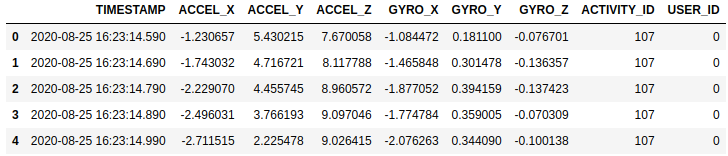
\includegraphics[width=1\textwidth, height=0.25\textheight]{Data.png}
	
	\caption{Πρώτες πέντε εγγραφές του πίνακας δεδομένων.}
	\label{plot:epoch-error}
\end{figure}
\noindent
όπου η κολόνα \en TIMESTAMP \gr αναφέρεται στο χρόνο δειγματοληψίας της εγγραφής, η κολόνα \en ACCEL\_\{X,Y,Z\} \gr αναφέρεται στην μέτρηση του επιταχυνσιομέτρου στον άξονα \{$x, y, z$\}, η κολόνα \en GYRO\_\{X,Y,Z\} \gr αναφέρεται στην μέτρηση του γυροσκοπίου στον άξονα \{$x, y, z$\}, η κολόνα \en ACTIVITY\_ID \gr δηλώνει την δραστηριότητα που πραγματοποιεί ο χρήστης και τέλος η κολόνα \en USER\_ID \gr αναφέρεται στον ποίος χρήστης έκανε την δραστηριότητα. Οι μετρήσεις των αισθητήρων καταγράφουν δείγματα στον τρισδιάστατο χώρο, αυτός είναι και ο λόγος που κάθε αισθητήρας έχει μετρήσεις τριών τυχαίων μεταβλητών ($x, y, z$). Επίσης ο κάθε χρήστης έχει μοναδικό \en ID\gr. Πλέον τα δεδομένα έχουν κατασκευαστεί και αποθηκευτεί με τέτοιο τρόπο, ώστε να είναι έτοιμα για να χρησιμοποιηθούν για το πρόβλημα της αυτόματης ταξηνόμησης ακολουθίας $\{(X_{i}, y_{i})\}_{i=1}^{N}$, με κατηγορία $y_{i}$ για κάθε ακολουθία $X_{i}$. Η κάθε ακολουθία $X_{i}$ μοντελοποιείται σαν πολυδιάστατη χρονοσειρά αισθητηριακών σημάτων, έχοντας $Τ_{i}$ δείγματα $\left<x_{1}, x_{2}, ..., x_{T_{i}}\right>_{i}$, με κατηγορία δραστηριότητας $y_{i}$. Τέλος τo κάθε δείγμα $x_{j} = [ACCEL\_X, ACCEL\_Y, ACCEL\_Z, GYRO\_X, GYRO\_Y, GYRO\_Z]_{j}$ και με $y_{j} = ACTIVITY\_ID$. Για την διαχείρηση των δεδομένων έγινε χρήση της βιβλιοθήκης \en pandas \gr \cite{reback2020pandas}.

\section{Αυτόματη Kατάτμηση}
Μετά την συλλογή των δεδομένων που μοντελοποιούνται σαν πολυδιάστατη χρονοσειρά αισθητηριακών σημάτων ακολουθεί η προ-επεξεργασία τους. Το πρώτο βασικό βήμα της προ-επεξεργασίας είναι η αυτόματη κατάτμηση του σήματος. Για την επίτευξη της αυτόματης κατάτμησης έγινε χρήση της συνάρτησης \en Segment(width, overlap) \gr της βιβλιοθήκης \en seglearn \cite{arXiv:1803.08118} \gr. Η συνάρτηση λαμβάνει ως είσοδο το αρχικό σήμα και το τμηματοποιεί σε τμήματα μεγέθους \en width\gr, κάνοντας χρήση ενός επικαλυπτόμενου κυλιόμενου παραθύρου (\en sliding window\gr) σταθερού μήκος, στην περίπτωσή μας το \en width \gr ίσο με 5 δευτερόλεπτα. Με αυτήν την μέθοδο κατασκευάζουμε ένα τρισδιάστατο χρονικό τένσορα $\phi_{i} = \left<W_{1}, ..., W_{M}\right>$ και για κάθε χρονοσειρά $X_{i}$. Ο τένσορας $\phi_{i}$ έχει σχήμα $\left(M_{i}, width, 6\right)$ με $width$ το μήκος του παραθύρου και $M_{i}$ ο αριθμός των παραθύρων που κατασκευάστηκαν για κάθε χρονοσειρά $X_{i}$. Το τελικό σύνολο δεδομένων είναι το σύνολο όλων των τμημάτων που παρήχθησαν από το κυλιόμενο παράθυρο και συμβολίζεται $\{W_{i}, y_{i}\}_{i=1}^{N_{w}}$, όπου το $N_{w}$ είναι το πλήθος των τμημάτων του συνόλου δεδομένων. Το πρόβλημα μηχανικής μάθησης της ταξινόμησης των πολυδιάστατων χρονοσειρών του έργου πλέον διατυπώθηκε και αξιολογήθηκε ως ταξινόμηση του τμηματοποιημένου συνόλου δεδομένων $\{W_{i}, y_{i}\}_{i=1}^{N_{w}}$.

\section{Εξαγωγή Χαρακτηριστικών}
Το επόμενο βήμα είναι η εξαγωγή των χαρακτηριστικών $F = \mathcal{F}(W)$ του τμηματοποιημένου συνόλου δεδομένων $\{W_{i}, y_{i}\}_{i=1}^{N_{w}}$. Πιο συγκεκριμένα για κάθε τμήμα $W_{i}$ θα εξαγάγουμε κάποια στατιστικά μεγέθη τα οποία στην συνέχεια θα αποτελέσουν την είσοδο για τον αλγόριθμο της μηχανικής μάθησης. Με αυτήν την ενέργεια από τον χώρο του τμηματοποιημένου σήματος $\{W_{i}, y_{i}\}_{i=1}^{N_{w}}$, μεταφερόμαστε στον χώρο των χαρακτηριστικών $\{F_{i}, y_{i}\}_{i=1}^{N_{w}}$. Αυτή η διαδικασία γίνεται για κάθε τυχαία μεταβλητή του τμήματος $W_{i}$ ξεχωριστά. Μερικά από τα χαρακτηριστικά (στατιστικά μεγέθη) που χρησιμοποιήθηκαν είναι η μέση τιμή, η διάμεσος, το άθροισμα των τετραγώνων, η τυπική απόκλιση, η διακύμανση, το μέγιστο και ελάχιστο στοιχείο, η λοξότητα, η κύρτωση, η μέση φασματική ενέργεια, το μέσο όρο των απόλυτων τιμών, η ρίζα των μέσων τετραγώνων κα.

%Τα χαρακτηριστικά που χρησιμοποιήθηκαν παρατίθενται στον παρακάτω πίνακα: 

%\begin{table}[h]
%	\centering
%	\begin{tabular}{| c | | c | | c |}
%		\hline
%		Στατιστικό μέγεθος & Σύμβολο & Τύπος\\ 
%		\hline
		
%		\hline
%		Μέσος όρος & $\mu$ & $\frac{1}{n} \sum\limits_{i=1}^{n} x_{i}$\\ 
%		
%		\hline
%		Διάμεσος & - & -\\ 
		
%		\hline
%		Τυπική απόκλιση & $\sigma$ & $\sqrt{\frac{1}{n}\sum\limits_{i=1}^{n} \left(x_{i} - \mu\right)^{2}}$ \\ 
		
%		\hline
%		Διακύμανση & $\sigma^{2}$ & $\frac{1}{n}\sum\limits_{i=1}^{n} \left(x_{i} - \mu\right)^{2}$ \\ 
		
%		\hline
%		Ελάχιστη τιμή & $\min$ & $\min(x)$ \\
		
%		\hline
%		Μέγιστη τιμή & $\max$ & $\max(x)$ \\
		
%		\hline
%		Άθροισμα τετραγώνων & - & $\sum\limits_{i=1}^{n} x_{i}^{2}$ \\ 
		
%		\hline
%	\end{tabular}
%	\caption{Χαρακτηριστικά.}
%	\label{tab:Features}
%\end{table}

\section{Προ-επεξεργασία Χαρακτηριστικών}
Στην συνέχεια ακολούθησε η κανονικοποίηση των δεδομένων εκπαίδευσης που πλέον είναι τα χαρακτηριστικά που εξαγάγαμε στο προηγούμενο βήμα. Η κανονικοποίηση του συνόλου δεδομένων είναι μια κοινή απαίτηση για πολλούς εκτιμητές μηχανικής μάθησης. Συνήθως αυτό γίνεται αφαιρώντας το μέσο όρο και κλιμακώνοντας τη διακύμανση στη μονάδα. Ωστόσο, οι υπερβολικές τιμές (τα \en outliers \gr) μπορούν συχνά να επηρεάσουν τη μέση τιμή και την διακύμανση του δείγματος με αρνητικό τρόπο. Για την αντιμετώπιση αυτού το προβλήματος σε αυτό το βήμα διαλέχτηκε η μέθοδος του \en robust data scaling \gr της βιβλιοθήκης \en scikit-learn \gr \cite{scikit-learn} καθώς αγνοεί τις ακραίες τιμές και παρήγαγε τα καλύτερα αποτελέσματα σε σχέση με άλλες μεθόδους κανονικοποίησης που δοκιμάστηκαν. Για να το πετύχει αυτό ο συγκεκριμένος μετασχηματισμός λειτουργεί αφαιρώντας την διάμεσο από του χαρακτηριστικού και στην συνέχεια διαιρώντας ενδοτεταρτημοριακό εύρος του \en(interquartile range)\gr.

\section{Μείωση της διάστασης}

\section{Το μοντέλο}
Πλέον μετά από τα στάδια διαλογής και προ-επεξεργασία των δεδομένων, συνεχίζουμε στον ορισμό του μοντέλου μηχανικής μάθησης με στόχο την αυτόματη κατηγοριοποίηση (ταξινόμηση) της πολυδιάστατης χρονοσειράς των αισθητηριακών σημάτων.
\begin{figure}[H]
\centering
	\begin{tikzpicture}[node distance=2cm]
	
	
	
		\node (stage0) [stage] {
			\begin{tabular}{c}
				Αρχικά Δεδομένα\\
				$\{(X_{i}, y_{i})\}_{i=1}^{N}$\\
			\end{tabular}
		};
		
		\node (stage1) [stage, below of=stage0] {
			\begin{tabular}{c}
				Τμηματοποιημένα Δεδομένα\\
				$\{W_{i}, y_{i}\}_{i=1}^{N_{w}}$\\
			\end{tabular}
		};
	
		\node (stage2) [stage, below of=stage1] {
			\begin{tabular}{c}
				Εξαγωγή Χαρακτηριστικών\\
				$\{F_{i}, y_{i}\}_{i=1}^{N_{w}}$\\
			\end{tabular}
		};
		
		\node (stage3) [stage, below of=stage2] {
			\begin{tabular}{c}
				Κανονικοποίηση Χαρακτηριστικών\\
				\en Robust Scaler \gr\\
			\end{tabular}
		};
		
		\node (stage4) [stage, below of=stage3] {
			\begin{tabular}{c}
				Μείωση της Διάστασης\\
				\en PCA \gr\\
			\end{tabular}
		};
		
		\node (stage5) [stage, below of=stage4] {
			\begin{tabular}{c}
				Μοντέλο Μηχανικής Μάθησης\\
				\en Logistic regression \gr\\
			\end{tabular}
		};
		
		\draw [arrow] (stage0) -- (stage1);
		\draw [arrow] (stage1) -- (stage2);
		\draw [arrow] (stage2) -- (stage3);
		\draw [arrow] (stage3) -- (stage4);
		\draw [arrow] (stage4) -- (stage5);
	\end{tikzpicture}
	\caption{Αλυσίδα αυτόματης κατάτμησης \& κατηγοριοποίησης της πολυδιάστατης χρονοσειράς αισθητηριακών σημάτων.}
\end{figure}

\section{Αξιολόγηση}

%\addstarredchapterc{\bibname} % minitoc
\en
\bibliographystyle{ieeetr}
\bibliography{Bibliography}

\end{document}